\chapter{生命的基本单位}\label{ch:b1:cell-unit-of-life}

1665 年，胡克把一小片软木放到透镜下，看到它被分隔成许多
微小的小格子，他称之为\omterm{def:b1:cell-unit-of-life:cell}{细胞}，这个名字取自修道院中的小房间。
十年后，荷兰布商列文虎克亲手磨制透镜，
\omterm{def:b1:cell-unit-of-life:resolution}{放大}能力超过当时的任何人，他看到活的生物
在一滴池水中游动，在他刮下的牙垢里，在他自己的
精液里。此后又过了一个半世纪，人们才归纳出两人所见的结论：
每个\omterm{def:b1:organism-environment:organism}{生物体}都由\omterm{def:b1:cell-unit-of-life:cell}{细胞}构成，
每个\omterm{def:b1:cell-unit-of-life:cell}{细胞}都来自另一个\omterm{def:b1:cell-unit-of-life:cell}{细胞}。本章阐述\omterm{prop:b1:cell-unit-of-life:theory}{细胞学说}及其依据，
比较两类\omterm{def:b1:cell-unit-of-life:cell}{细胞}，并介绍
这些仪器：显微镜、离心机和培养瓶——
它们让我们能观察\omterm{def:b1:cell-unit-of-life:cell}{细胞}、拆开\omterm{def:b1:cell-unit-of-life:cell}{细胞}，并使\omterm{def:b1:cell-unit-of-life:cell}{细胞}
在\omterm{def:b1:organism-environment:organism}{生物体}外保持存活。

\section{细胞学说}

\begin{definition}[细胞]\label{def:b1:cell-unit-of-life:cell}
称\emph{细胞}\index{细胞}为最小的活物质单位：一团
由含水的\emph{细胞质}\index{细胞质}构成的一定体积，
由\emph{质膜}\index{质膜}包围，内含遗传物质，
即 DNA 以及表达它的机制，能够摄取营养物质、
转化能量、维持自身的\omterm{def:b1:body-plans-tissues:tissue}{组织}，并在条件允许时
分裂为两个细胞。
\end{definition}

\begin{proposition}[细胞学说]\label{prop:b1:cell-unit-of-life:theory}
\index{细胞学说}
\begin{enumerate}
  \item 每个\omterm{def:b1:organism-environment:organism}{生物体}都由一个或多个\omterm{def:b1:cell-unit-of-life:cell}{细胞}构成，\omterm{def:b1:cell-unit-of-life:cell}{细胞}是
        生物结构与功能的基本单位
        （施莱登和施旺，1838--1839）。
  \item 每个\omterm{def:b1:cell-unit-of-life:cell}{细胞}都由已存在的\omterm{def:b1:cell-unit-of-life:cell}{细胞}通过分裂产生
        （菲尔绍，1855：\emph{omnis cellula e cellula}）；不存在
        自发生成。
  \item 遗传物质在分裂时由\omterm{def:b1:cell-unit-of-life:cell}{细胞}传给\omterm{def:b1:cell-unit-of-life:cell}{细胞}，
        因而生命的连续性
        即\omterm{def:b1:cell-unit-of-life:cell}{细胞}的连续性。
\end{enumerate}
\end{proposition}
\begin{proof}[证据]
胡克的软木（1665 年）以及格鲁和马尔皮基的植物切片显示
植物\omterm{def:b1:body-plans-tissues:tissue}{组织}为成排的小室；列文虎克的透镜（1670 年代）显示
单\omterm{def:b1:cell-unit-of-life:cell}{细胞}生物、血\omterm{def:b1:cell-unit-of-life:cell}{细胞}和精子。两个世纪的
透镜改进使人们在所检查的每一种\omterm{def:b1:body-plans-tissues:tissue}{组织}中都发现了\omterm{def:b1:cell-unit-of-life:cell}{细胞}，动物与
植物皆然，施旺在软骨和胚胎中认出有核\omterm{def:b1:cell-unit-of-life:cell}{细胞}。
人们直接观察到藻类和胚胎中的分裂，菲尔绍发现
没有哪一种\omterm{def:b1:body-plans-tissues:tissue}{组织}，无论健康或患病，其\omterm{def:b1:cell-unit-of-life:cell}{细胞}不是来自其他
\omterm{def:b1:cell-unit-of-life:cell}{细胞}。巴斯德的鹅颈瓶（1861 年）中，肉汤
在灰尘无法进入时数月保持无菌，在灰尘进入后
数日内便滋生，由此终结了自发生成的问题。第三条
论断属于十九世纪后期的工作，那时人们
追踪了分裂过程中的染色体（\cref{ch:b1:replication-mitosis}）。
\end{proof}

\begin{omfigure}
\begin{minipage}[b]{0.46\linewidth}\centering
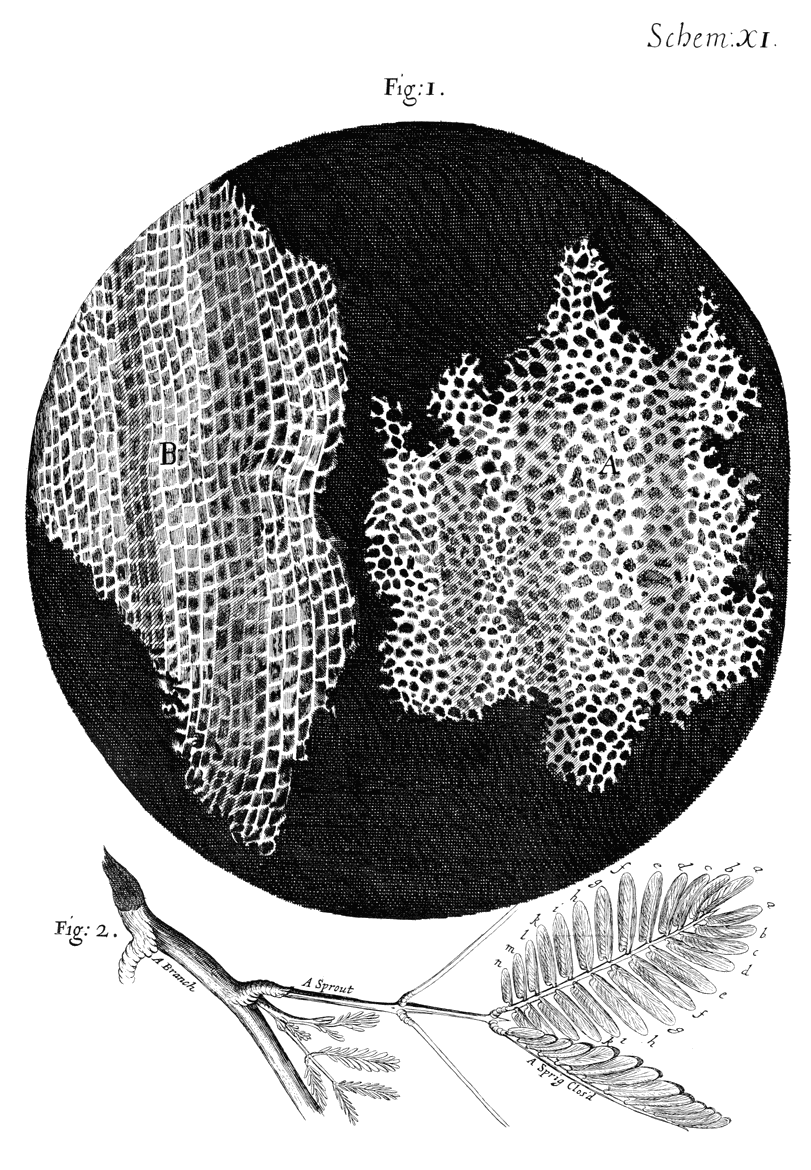
\includegraphics[width=0.9\linewidth]{images/book3/hooke-cork.png}
\end{minipage}\hfill
\begin{minipage}[b]{0.46\linewidth}\centering
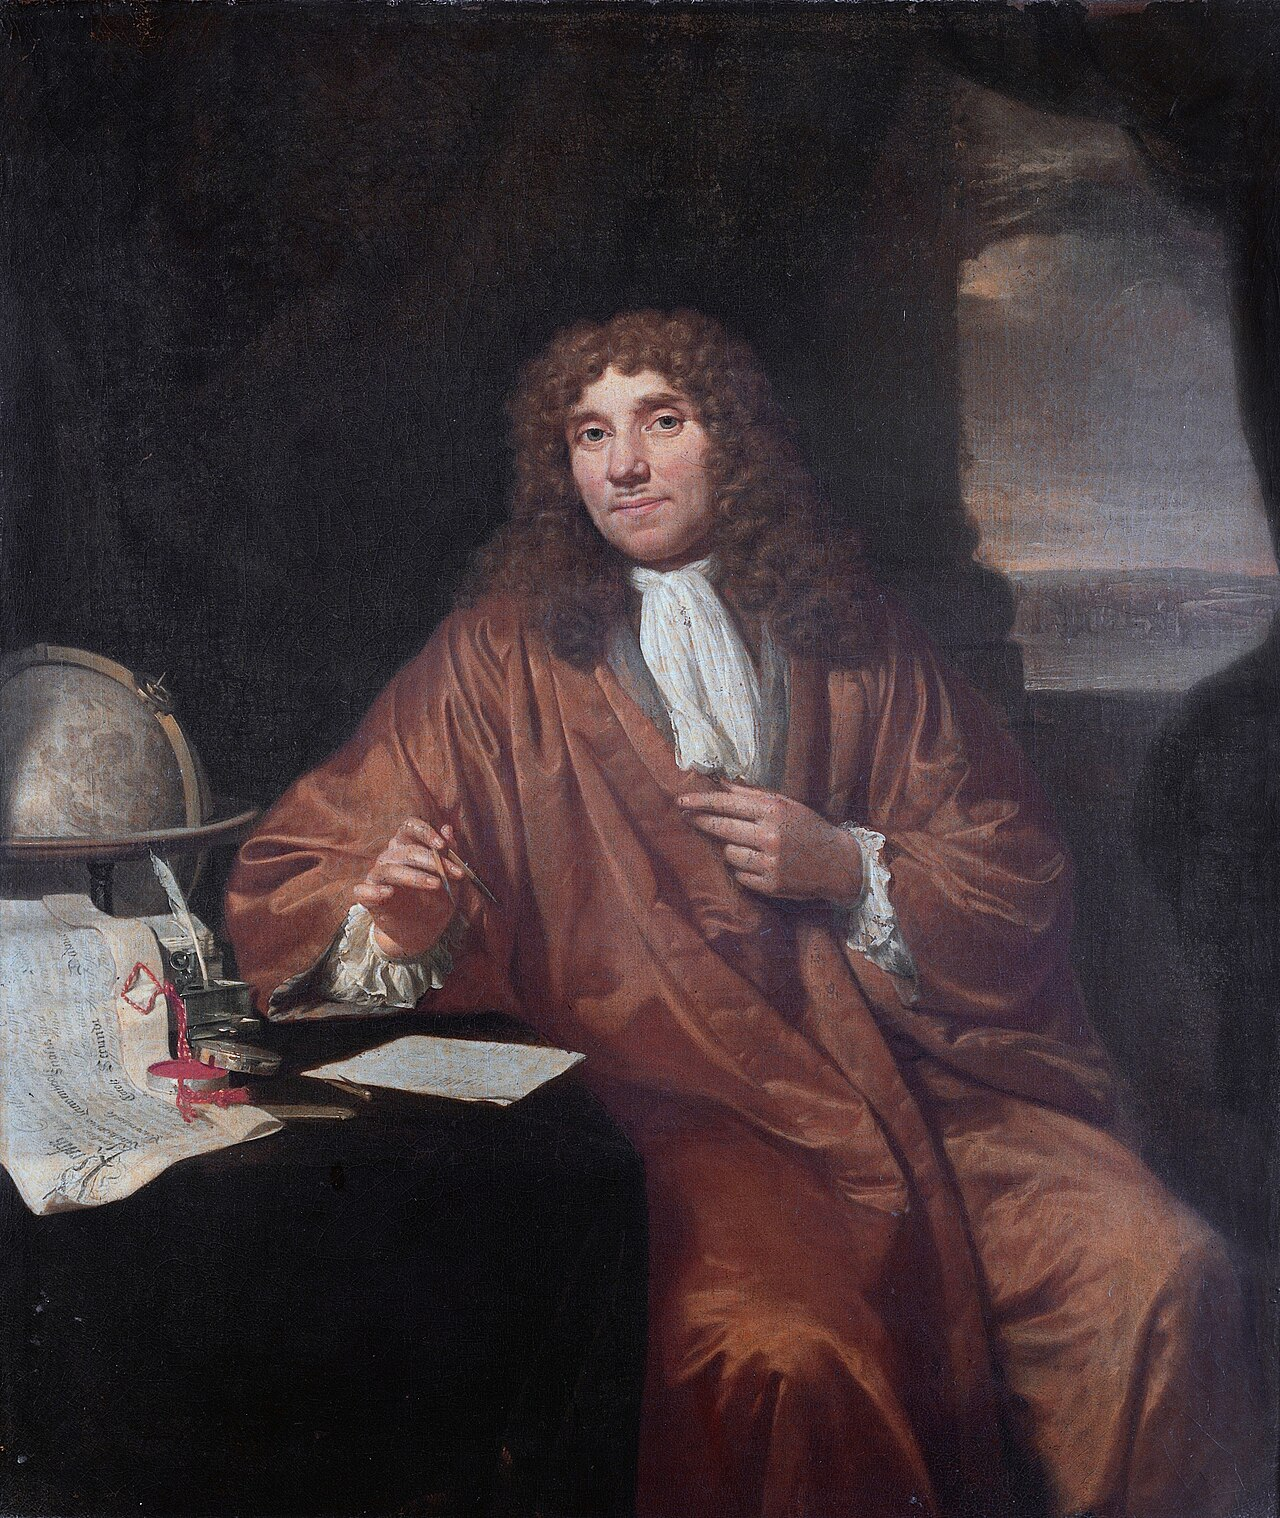
\includegraphics[width=0.78\linewidth]{images/book3/leeuwenhoek.jpg}
\end{minipage}

{\small 左：胡克在 \emph{Micrographia}（1665）中绘制的软木图，
这是最早被绘出的\omterm{def:b1:cell-unit-of-life:cell}{细胞}——死\omterm{def:b1:cell-unit-of-life:cell}{细胞}空的\omterm{def:b1:cell-unit-of-life:prokeuk}{细胞壁}，从
两个方向。右：列文虎克像，由扬·韦尔科耶绘制，
时间约为 1680 年，其单透镜显微镜首次显示了
活\omterm{def:b1:cell-unit-of-life:cell}{细胞}。}
\end{omfigure}

\begin{example}[单细胞与多细胞]\label{ex:b1:cell-unit-of-life:onemany}
细菌、酵母与变形虫都是单\omterm{def:b1:cell-unit-of-life:cell}{细胞}生物，独自
完成摄食、运动、分裂等一切活动，尺度只有几微米。
人体约含 $\num{3e13}$ 个\omterm{def:b1:cell-unit-of-life:cell}{细胞}，分为两百种，其中任何一种都不能
单独在池塘中生存，每个\omterm{def:b1:cell-unit-of-life:cell}{细胞}都经由不间断的
分裂，追溯到同一个受精卵。兔子的情形见
\cref{ch:b1:mammal-organization}，橡树的情形见
\cref{ch:b1:flowering-plant-organization}，两者
都是同一理论的两次应用。
\end{example}

\section{两类细胞}

\begin{definition}[原核细胞与真核细胞]\label{def:b1:cell-unit-of-life:prokeuk}
称\emph{原核细胞}\index{原核细胞}（细菌、古菌）
没有\omterm{def:b1:cell-unit-of-life:cell}{细胞}核，其 DNA（通常为一条环状染色体）位于
\omterm{def:b1:cell-unit-of-life:cell}{细胞质}中一个称为\emph{拟核}\index{拟核}的区域，
\omterm{def:b1:cell-unit-of-life:cell}{细胞}内没有膜包被的区室。体积很小，
（\qtyrange{0.5}{5}{\micro m}），由\omterm{def:b1:cell-unit-of-life:cell}{质膜}包被，
其外为\emph{细胞壁}\index{细胞壁}。\emph{真核
细胞}\index{真核细胞}（原生生物、真菌、植物和动物）的
DNA 以数条线性染色体的形式，位于
\emph{细胞核}\index{细胞核}内，该核由双层膜包被，并将
\omterm{def:b1:cell-unit-of-life:cell}{细胞质}分隔成由膜包围的\emph{细胞器}\index{细胞器}
（\cref{ch:b1:eukaryotic-cell}）。其体积较大，
（\qtyrange{10}{100}{\micro m}），内部具有由蛋白质
纤维构成的骨架。
\end{definition}

\begin{omfigure}
\begin{tikzpicture}
  \node[anchor=south west, inner sep=0] (img) at (0,0)
    {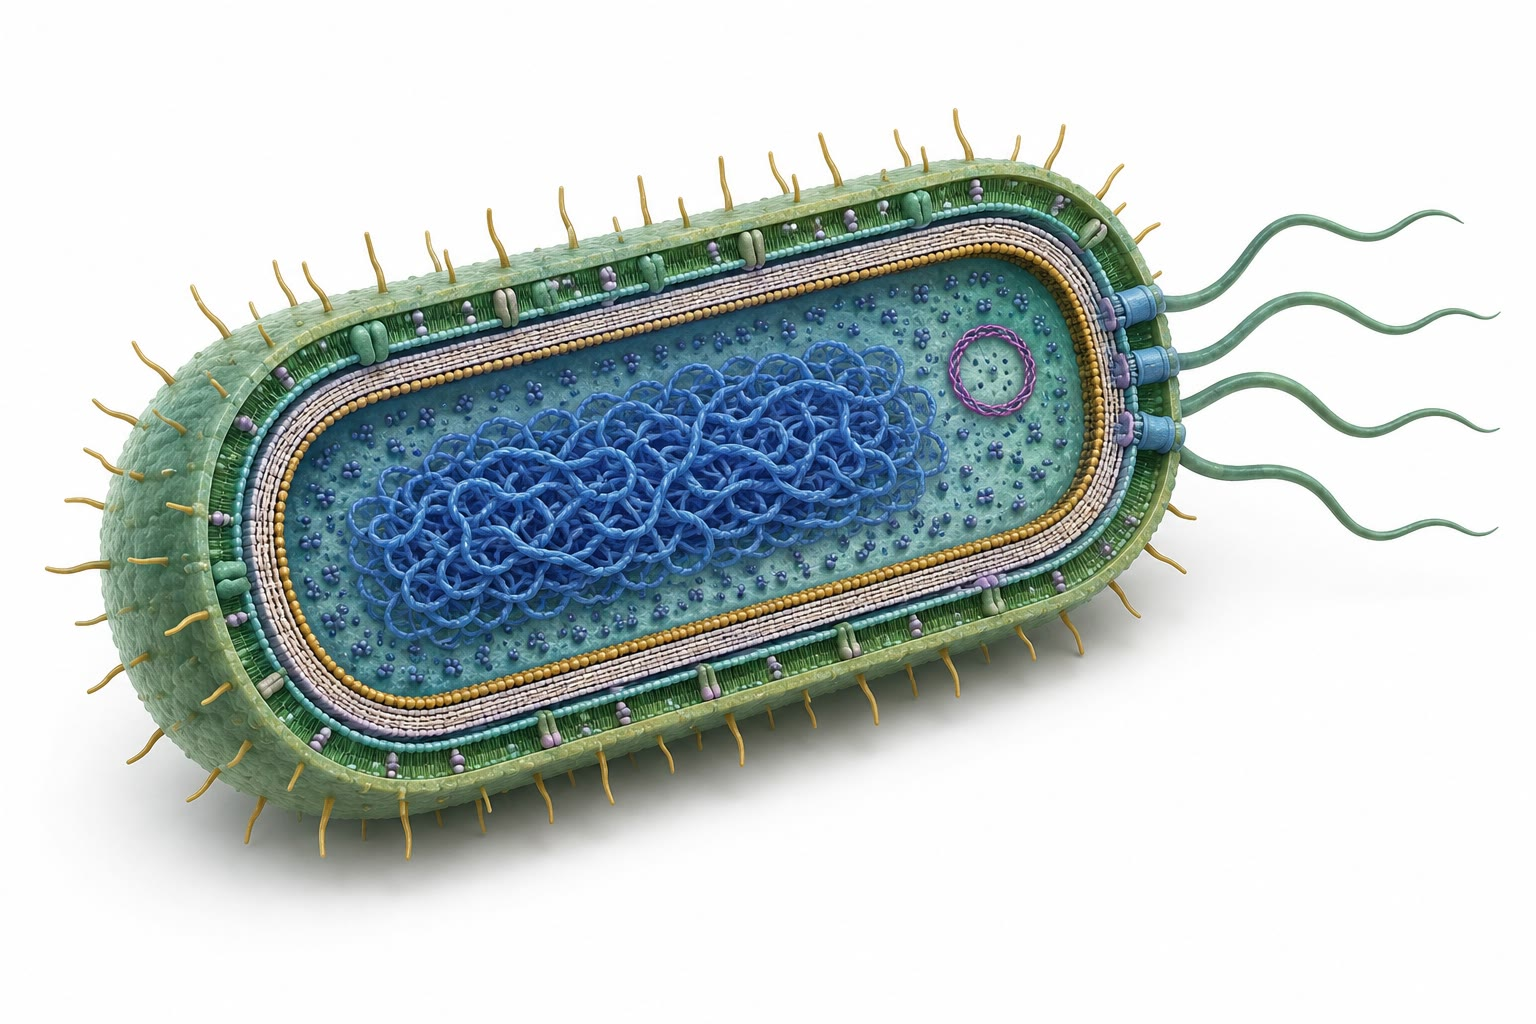
\includegraphics[width=0.54\linewidth]{images/book3/ai/fig-ecoli-cell.jpg}};
  \begin{scope}[x={(img.south east)}, y={(img.north west)},
      every node/.style={font=\small}]
    \draw[omDef, thick] (0.45,0.52) -- (0.45,1.08) node[above] {拟核：环状 DNA};
    \draw[omDef, thick] (0.75,0.55) -- (1.03,0.46) node[right] {核糖体};
    \draw[omDef, thick] (0.17,0.45) -- (-0.03,0.40) node[left, align=right] {细胞壁和 \\ 两层膜};
    \draw[omDef, thick] (0.65,0.64) -- (1.03,0.24) node[right] {质粒};
    \draw[omDef, thick] (0.88,0.68) -- (1.03,0.80) node[right] {鞭毛};
    \draw[omDef, thick] (0.35,0.19) -- (0.35,-0.08) node[below] {菌毛};
  \end{scope}
\end{tikzpicture}

{\small 细菌（\emph{Escherichia coli}）剖面图。无\omterm{def:b1:cell-unit-of-life:prokeuk}{细胞核}，无
\omterm{def:b1:cell-unit-of-life:prokeuk}{细胞器}：一条环状染色体松散地折叠于\omterm{def:b1:cell-unit-of-life:cell}{细胞质}中，
数千个核糖体之间；\omterm{def:b1:cell-unit-of-life:cell}{质膜}外为\omterm{def:b1:cell-unit-of-life:prokeuk}{细胞壁}，鞭毛用于
游动，菌毛用于附着。长约 \qty{2}{\micro m}。}
\end{omfigure}

\begin{omfigure}
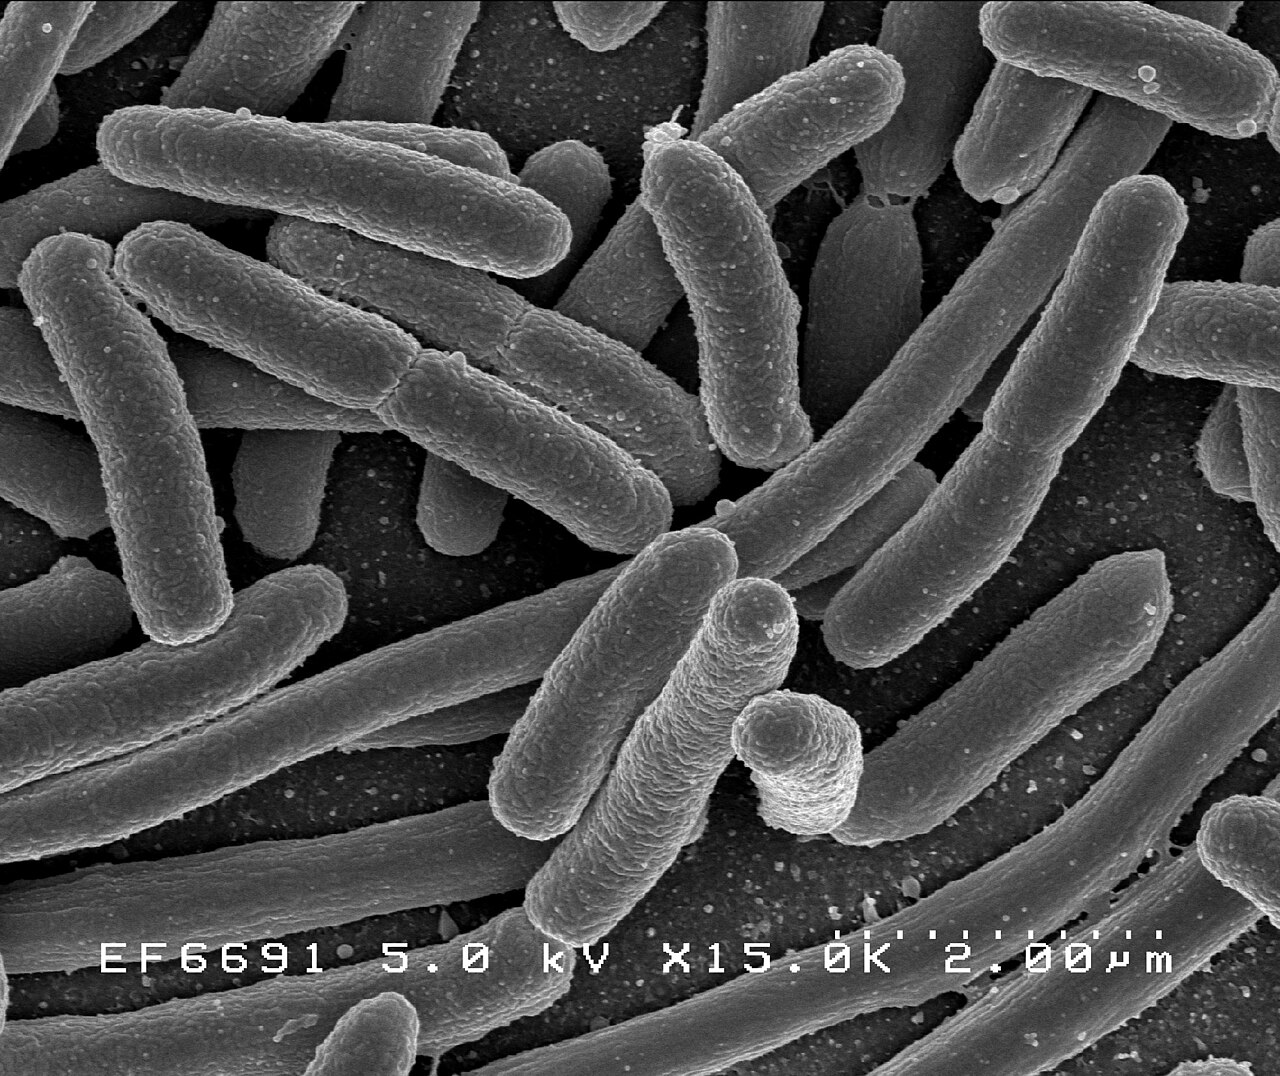
\includegraphics[width=0.5\linewidth]{images/book3/ecoli-niaid.jpg}

{\small 扫描\omterm{prop:b1:cell-unit-of-life:microscopes}{电子显微镜}下的 \emph{Escherichia coli}
（图像底部标尺为 \qty{2}{\micro m}）。杆状菌体长
\qty{2}{\micro m}，一千个并排可跨越一
毫米；单个\omterm{def:b1:cell-unit-of-life:cell}{细胞}在营养丰富的
培养基中每二十分钟分裂一次。图片：NIAID，公有领域。}
\end{omfigure}

\begin{proposition}[细菌细胞]\label{prop:b1:cell-unit-of-life:bacterium}
\emph{E. coli} 是模式细菌，为杆状，长 \qty{2}{\micro m}，
宽 \qty{0.8}{\micro m}：体积约为 \qty{1}{\micro m^3}，内含
一条含 $\num{4.6e6}$ 个碱基对的染色体（\qty{1.5}{mm} 长的 DNA
经折叠压缩了一万倍），约 \num{20000} 个核糖体，数百万个蛋白质
分子，共 \num{2000} 种，并常含一个或多个
\emph{质粒}\index{质粒}——小型环状 DNA 分子，携带
额外基因。其包膜由内向外依次为\omterm{def:b1:cell-unit-of-life:cell}{质膜}、
一层薄的\emph{肽聚糖}\index{肽聚糖}壁（由糖链经短肽交联而成的网状结构，
能抵抗\omterm{def:b1:cell-unit-of-life:cell}{细胞}的内部压力），
以及外膜。肽聚糖壁厚、无外膜的
细菌保留了\emph{革兰氏染色}\index{革兰氏染色}中的结晶紫
（革兰氏阳性）；
薄壁且具外膜的细菌则失去结晶紫（革兰氏阴性，如
\emph{E. coli}）。鞭毛如螺旋桨般转动；菌毛使\omterm{def:b1:cell-unit-of-life:cell}{细胞}附着于
表面及其他\omterm{def:b1:cell-unit-of-life:cell}{细胞}。
\end{proposition}

\begin{method}[革兰氏染色]\label{met:b1:cell-unit-of-life:gram}
\begin{enumerate}
  \item 加热将细菌薄涂片固定于载玻片上。
  \item 先用结晶紫染色（所有\omterm{def:b1:cell-unit-of-life:cell}{细胞}呈紫色），再用碘液处理，
        碘与\omterm{def:b1:cell-unit-of-life:cell}{细胞}内的染料形成大型复合物。
  \item 用酒精冲洗：革兰氏阳性菌厚的肽聚糖壁
        收缩并把复合物留在\omterm{def:b1:cell-unit-of-life:cell}{细胞}内；革兰氏阴性菌的薄壁
        在酒精溶解外膜后，
        使复合物被洗脱。
  \item 用粉红色染料（番红）复染：革兰氏阳性\omterm{def:b1:cell-unit-of-life:cell}{细胞}
        呈紫色，革兰氏阴性\omterm{def:b1:cell-unit-of-life:cell}{细胞}呈粉红色。结果可预测\omterm{def:b1:cell-unit-of-life:prokeuk}{细胞壁}
        结构，以及对多种抗生素的敏感性。
\end{enumerate}
\end{method}

\begin{omfigure}
\begin{tikzpicture}
\begin{semilogxaxis}[
  width=0.94\linewidth, height=6.0cm,
  axis x line=bottom, axis y line=none,
  xmin=0.05, xmax=5000000, ymin=0, ymax=1.6,
  xlabel={大小（\unit{nm}）},
  xlabel style={font=\small, at={(axis description cs:0.5,-0.14)}, anchor=north},
  xtick={0.1,1,10,100,1000,10000,100000,1000000}, log ticks with fixed point,
  xticklabels={0.1,1,10,100,\qty{1}{\micro m},\qty{10}{\micro m},\qty{100}{\micro m},\qty{1}{mm}},
  tick label style={font=\small}, clip=false,
]
\addplot[only marks, mark=*, mark size=1.8pt, omDef] coordinates {(0.1,0.75) (1,0.75) (10,0.75) (30,0.75) (100,0.75) (1000,0.75) (4000,0.75) (20000,0.75) (100000,0.75) (1000000,0.75)};
\node[font=\scriptsize, anchor=west, rotate=65, inner sep=1pt] at (axis cs:0.1,0.82) {原子};
\node[font=\scriptsize, anchor=west, rotate=65, inner sep=1pt] at (axis cs:1,0.82) {葡萄糖};
\node[font=\scriptsize, anchor=west, rotate=65, inner sep=1pt] at (axis cs:10,0.82) {蛋白质};
\node[font=\scriptsize, anchor=west, rotate=65, inner sep=1pt] at (axis cs:30,0.82) {核糖体};
\node[font=\scriptsize, anchor=west, rotate=65, inner sep=1pt] at (axis cs:100,0.82) {病毒};
\node[font=\scriptsize, anchor=west, rotate=65, inner sep=1pt] at (axis cs:1000,0.82) {细菌};
\node[font=\scriptsize, anchor=west, rotate=65, inner sep=1pt] at (axis cs:4000,0.82) {线粒体};
\node[font=\scriptsize, anchor=west, rotate=65, inner sep=1pt] at (axis cs:20000,0.82) {动物细胞};
\node[font=\scriptsize, anchor=west, rotate=65, inner sep=1pt] at (axis cs:100000,0.82) {人卵细胞};
\node[font=\scriptsize, anchor=west, rotate=65, inner sep=1pt] at (axis cs:1000000,0.82) {蛙卵};
\draw[very thick, omThm] (axis cs:0.2,0.52) -- (axis cs:1000000,0.52) node[pos=0.5, above, font=\scriptsize, omThm, inner sep=1.5pt] {电子显微镜};
\draw[very thick, omProp] (axis cs:200,0.34) -- (axis cs:1000000,0.34) node[pos=0.5, above, font=\scriptsize, omProp, inner sep=1.5pt] {光学显微镜};
\draw[very thick, omExo] (axis cs:100000,0.16) -- (axis cs:5000000,0.16) node[pos=0.5, above, font=\scriptsize, omExo, inner sep=1.5pt] {肉眼};
\end{semilogxaxis}
\end{tikzpicture}

{\small 各种事物的大小（对数刻度），以及能\omterm{def:b1:cell-unit-of-life:resolution}{分辨}它们的
仪器。细菌恰好略高于\omterm{prop:b1:cell-unit-of-life:microscopes}{光学显微镜}的
\omterm{def:b1:cell-unit-of-life:resolution}{分辨}极限；\omterm{def:b1:cell-unit-of-life:prokeuk}{真核细胞}在每一维度上大十倍，
体积则大一千倍。}
\end{omfigure}

\begin{example}[为何真核细胞要分隔成区室]\label{ex:b1:cell-unit-of-life:whycompart}
一个 \qty{20}{\micro m} 的\omterm{def:b1:cell-unit-of-life:cell}{细胞}，体积为
细菌的一千倍，而其膜表面积仅为一百倍
（见\cref{prop:b1:organism-environment:sv}）。膜是\omterm{def:b1:cell-unit-of-life:cell}{细胞}承载
能量转换链与运输系统的场所；真核生物
通过在\omterm{def:b1:cell-unit-of-life:cell}{细胞}内部折叠膜来恢复表面积——
例如线粒体内膜、内质网的膜片，
还获得了彼此分隔的区室，
使互不相容的化学过程（溶酶体中的消化、
\omterm{def:b1:cell-unit-of-life:cell}{细胞}溶胶中的合成）得以并行进行。
\end{example}

\section{细胞观察：显微术}

\begin{definition}[放大率与分辨率]\label{def:b1:cell-unit-of-life:resolution}
显微镜能\emph{放大}\index{放大}（使图像变大）
并能\emph{分辨}\index{分辨}（区分相邻的两个点）。
只有后者限制了可见的范围：\emph{分辨
率}\index{分辨率}是两点之间的最小距离 $d$，
在此距离下两点仍可被区分为不同的点，
\[
d = \frac{0.61\,\lambda}{\mathrm{NA}},
\]
其中 $\lambda$ 为照明光的波长，$\mathrm{NA}$
为物镜的数值孔径（即其光收集半角的正弦
乘以介质的折射率，至多
约为 $1.4$（使用油浸时）。超出分辨率的放大
只会放大模糊，而非细节。
\end{definition}

\begin{proposition}[光学显微镜与电子显微镜]\label{prop:b1:cell-unit-of-life:microscopes}
用可见光（$\lambda \approx \qty{550}{nm}$）照明，
$\mathrm{NA} = 1.4$ 时，\emph{光学显微镜}\index{光学显微镜}可\omterm{def:b1:cell-unit-of-life:resolution}{分辨} \qty{0.24}{\micro m}：\omterm{def:b1:cell-unit-of-life:cell}{细胞}、\omterm{def:b1:cell-unit-of-life:prokeuk}{细胞核}、叶绿体、
线粒体（呈点状）、细菌（呈杆状）——以及活的、运动中的标本。
透明\omterm{def:b1:cell-unit-of-life:cell}{细胞}的反差可借助染色获得（染色通常会
杀死\omterm{def:b1:cell-unit-of-life:cell}{细胞}）、借助\emph{相差}（把折射率的差异转化为亮度的差异），
或借助\emph{荧光}
（用染料或荧光蛋白标记一个分子，仅成像其发出的光）。
\emph{电子显微镜}\index{电子显微镜}所用电子的波长仅为几皮米；其
实际\omterm{def:b1:cell-unit-of-life:resolution}{分辨率}受限于透镜，在透射模式下约为 \qty{0.2}{nm}，
（TEM：电子穿过厚度为 \qty{50}{nm} 的切片，经重金属染色后，
显示\omterm{def:b1:cell-unit-of-life:prokeuk}{细胞器}的内部结构），在扫描模式下为几纳米
（SEM：电子束扫过覆有金属镀层的表面，显示其深度上的起伏）。
电子显微术需要真空，
标本须已死亡、固定并脱水。
\end{proposition}

\begin{omfigure}
\begin{tikzpicture}[font=\footnotesize, >=Stealth, line cap=round]
  % optical axis
  \draw[gray, dashed] (0,0) -- (11.4,0);
  % object
  \draw[very thick, omExo, ->] (0.6,0) -- (0.6,0.35) node[above, font=\scriptsize] {物体};
  % objective lens
  \draw[very thick, omDef] (2.0,-0.9) .. controls (2.35,0) .. (2.0,0.9);
  \draw[very thick, omDef] (2.0,-0.9) .. controls (1.65,0) .. (2.0,0.9);
  \node[below, font=\scriptsize] at (2.0,-1.0) {物镜};
  % intermediate image
  \draw[very thick, omExo, ->] (6.2,0) -- (6.2,-1.4) node[below, font=\scriptsize] {中间像（倒立、放大）};
  % eyepiece
  \draw[very thick, omDef] (8.4,-0.9) .. controls (8.75,0) .. (8.4,0.9);
  \draw[very thick, omDef] (8.4,-0.9) .. controls (8.05,0) .. (8.4,0.9);
  \node[above, font=\scriptsize] at (8.4,1.0) {目镜};
  % eye
  \draw[thick] (10.6,0) circle (0.35); \node[font=\scriptsize, above] at (10.6,0.45) {眼睛};
  % rays: from object tip through objective to image tip
  \draw[omThm, thick] (0.6,0.35) -- (2.0,0.35) -- (6.2,-1.4);
  \draw[omThm, thick] (0.6,0.35) -- (2.0,-0.55) -- (6.2,-1.4);
  % rays from image tip through eyepiece, emerging parallel (virtual image at infinity)
  \draw[omThm, thick] (6.2,-1.4) -- (8.4,-0.6) -- (10.3,-0.15);
  \draw[omThm, thick] (6.2,-1.4) -- (8.4,0.5) -- (10.3,0.25);
  \node[align=center, font=\scriptsize, gray] at (4.2,1.2) {放大率 = 物镜 $\times$ 目镜 \\ 例如 $100\times$ 油浸物镜 $\times 10\times$ 目镜 $= 1000\times$};
\end{tikzpicture}

{\small 复式\omterm{prop:b1:cell-unit-of-life:microscopes}{光学显微镜}：物镜形成一个
\omterm{def:b1:cell-unit-of-life:resolution}{放大}的倒立中间像，目镜将其再次
\omterm{def:b1:cell-unit-of-life:resolution}{放大}供眼睛观察。物镜的数值孔径，而非总\omterm{def:b1:cell-unit-of-life:resolution}{放大}率，
决定可\omterm{def:b1:cell-unit-of-life:resolution}{分辨}的细节。}
\end{omfigure}

\begin{omfigure}
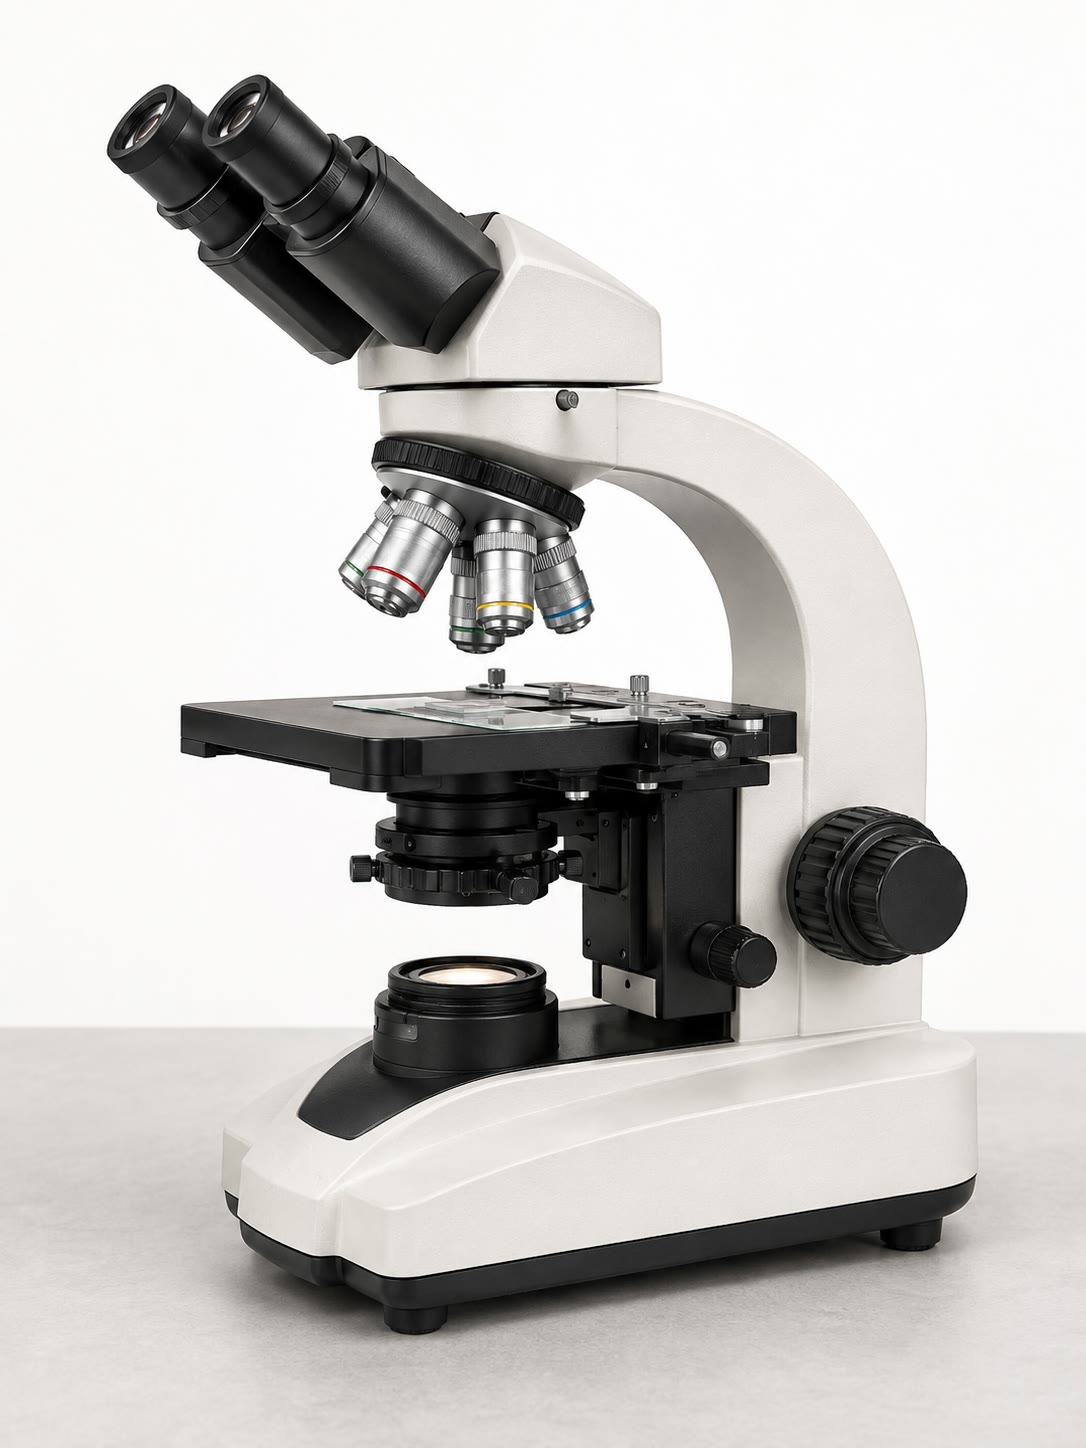
\includegraphics[width=0.36\linewidth]{images/book3/ai/b3-05-light-microscope.jpg}

{\small 复式\omterm{prop:b1:cell-unit-of-life:microscopes}{光学显微镜}：载物台下方为光源和冷凝器，
载物台上方为物镜转换盘，目镜为双目。\omterm{def:b1:cell-unit-of-life:resolution}{分辨率}
\qty{0.2}{\micro m}，\omterm{def:b1:cell-unit-of-life:resolution}{放大}率最高可达 \qty{1000}{}，活体标本
亦可观察。}
\end{omfigure}

\begin{method}[选择仪器]\label{met:b1:cell-unit-of-life:choose}
\begin{enumerate}
  \item 追踪活的过程（\omterm{def:b1:cell-unit-of-life:cell}{细胞}分裂、运动、荧光蛋白
        在各隔室之间的移动）：在未固定的\omterm{def:b1:cell-unit-of-life:cell}{细胞}上，使用
        光学显微术，配合相差或荧光观察。
  \item 计数并鉴定\omterm{def:b1:body-plans-tissues:tissue}{组织}中的\omterm{def:b1:cell-unit-of-life:cell}{细胞}：使用固定、切片的
        染色制片，在\omterm{prop:b1:cell-unit-of-life:microscopes}{光学显微镜}下观察。
  \item 观察\omterm{def:b1:cell-unit-of-life:prokeuk}{细胞器}、膜及病毒的内部结构：
        采用透射电子显微术观察薄切片，或
        观察经负染色的颗粒。
  \item 观察\omterm{def:b1:cell-unit-of-life:cell}{细胞}或\omterm{def:b1:body-plans-tissues:tissue}{组织}的表面形貌：
        采用扫描电子显微术。
  \item 定位某一种蛋白质：免疫荧光（光学）或
        免疫金标记（电子），均使用针对该蛋白质的抗体。
\end{enumerate}
\end{method}

\begin{example}[一个细菌与一个线粒体]\label{ex:b1:cell-unit-of-life:seeing}
在 $1000\times$ 的\omterm{prop:b1:cell-unit-of-life:microscopes}{光学显微镜}下，\emph{E. coli} \omterm{def:b1:cell-unit-of-life:cell}{细胞}
呈杆状，在视网膜尺度上长 \qty{2}{mm}，内部看不到结构；
线粒体则只是处于\omterm{def:b1:cell-unit-of-life:resolution}{分辨}极限处的一个点。在 TEM 切片中，
同一细菌可见其双层膜、\omterm{def:b1:cell-unit-of-life:prokeuk}{细胞壁}、呈淡色纤维状区域的\omterm{def:b1:cell-unit-of-life:prokeuk}{拟核}，
以及呈深色颗粒状的核糖体；
线粒体则可见其双层膜及内膜的褶皱。
两者都不是活的。
\end{example}

\section{拆分细胞与保持细胞存活}

\begin{definition}[细胞分级分离]\label{def:b1:cell-unit-of-life:fractionation}
\emph{细胞分级分离}\index{细胞分级分离}用于将\omterm{def:b1:cell-unit-of-life:cell}{细胞}的
各组分分离开以便研究。\omterm{def:b1:body-plans-tissues:tissue}{组织}先被制成
\emph{匀浆}\index{匀浆}——即在低温的
等渗缓冲液中通过研磨或剪切打破\omterm{def:b1:cell-unit-of-life:cell}{细胞}，使\omterm{def:b1:cell-unit-of-life:prokeuk}{细胞器}保持完整——
然后对匀浆进行\emph{差速
离心}\index{差速离心}：一系列离心，
离心力与时长逐级增加，每次离心都使悬浮液中残余的最大、
最致密的颗粒沉淀下来。每一组分
通过其在\omterm{prop:b1:cell-unit-of-life:microscopes}{电子显微镜}下的形态，以及
\emph{标志酶}\index{标志酶}，即已知仅存在于
某一隔室中的活性。
\end{definition}

\begin{omfigure}
\begin{tikzpicture}[font=\footnotesize, >=Stealth, line cap=round,
  tube/.style={draw, thick, rounded corners=2pt, minimum width=20mm, minimum height=9mm, align=center, fill=white},
  pel/.style={draw, thick, rounded corners=3pt, text width=29mm, minimum height=10mm, align=center, fill=omProp!15}]
  \node[tube, fill=omDef!10] (h) at (0,0) {匀浆};
  \node[tube, fill=omDef!10] (s1) at (3.5,0) {上清液 1};
  \node[tube, fill=omDef!10] (s2) at (7.0,0) {上清液 2};
  \node[tube, fill=omDef!10] (s3) at (10.5,0) {上清液 3};
  \node[tube, fill=omExo!15] (cy) at (13.6,0) {细胞溶胶};
  \draw[->, thick] (h) -- (s1) node[midway, above, align=center, font=\scriptsize] {$1000\,g$\\ \qty{10}{min}};
  \draw[->, thick] (s1) -- (s2) node[midway, above, align=center, font=\scriptsize] {$\num{10000}\,g$\\ \qty{20}{min}};
  \draw[->, thick] (s2) -- (s3) node[midway, above, align=center, font=\scriptsize] {$\num{100000}\,g$\\ \qty{60}{min}};
  \draw[->, thick] (s3) -- (cy) node[midway, above, align=center, font=\scriptsize] {无 \\ 沉淀};
  \node[pel] (p1) at (1.75,-1.9) {沉淀 1：细胞核、未破碎的细胞、碎片};
  \node[pel] (p2) at (5.25,-1.9) {沉淀 2：线粒体、溶酶体、过氧化物酶体};
  \node[pel] (p3) at (8.75,-1.9) {沉淀 3：微粒体（ER 片段）、核糖体};
  \draw[->, thick] (1.75,-0.5) -- (p1);
  \draw[->, thick] (5.25,-0.5) -- (p2);
  \draw[->, thick] (8.75,-0.5) -- (p3);
  \node[align=left, gray, anchor=north west, font=\scriptsize] at (10.4,-1.3) {标志物：DNA（细胞核）、\\ 琥珀酸脱氢酶 \\（线粒体）、酸性 \\ 磷酸酶（溶酶体）、\\ 葡萄糖-6-磷酸酶（ER）、\\ 乳酸脱氢酶（细胞溶胶）};
\end{tikzpicture}

{\small \omterm{def:b1:cell-unit-of-life:fractionation}{匀浆}的\omterm{def:b1:cell-unit-of-life:fractionation}{差速离心}。每次离心都使比前一次更大或更重的组分沉淀，
其余的留在悬液中：先是\omterm{def:b1:cell-unit-of-life:prokeuk}{细胞核}，然后是线粒体，
再是膜碎片，
最后是可溶的\omterm{def:b1:cell-unit-of-life:cell}{细胞}溶胶。\omterm{def:b1:cell-unit-of-life:fractionation}{标志酶}可以说明各\omterm{def:b1:cell-unit-of-life:prokeuk}{细胞器}
去向何处。}
\end{omfigure}

\begin{omfigure}
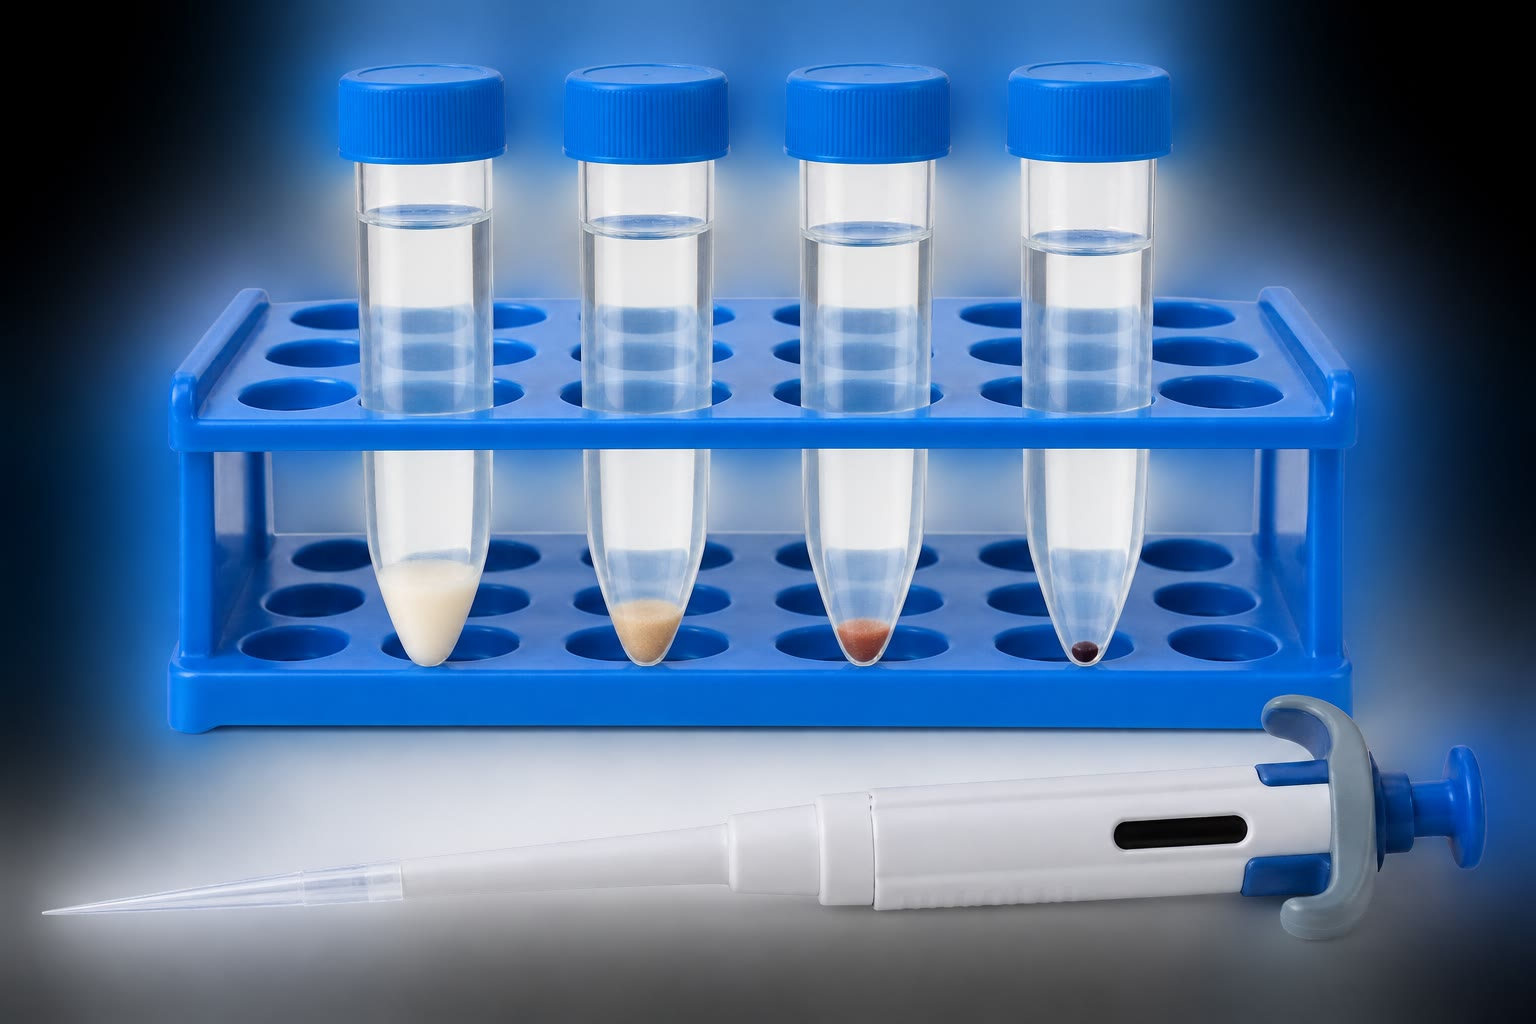
\includegraphics[width=0.5\linewidth]{images/book3/ai/b3-05-fractionation-tubes.jpg}

{\small 连续离心后的各组分：\omterm{def:b1:cell-unit-of-life:prokeuk}{细胞核}、
线粒体和微粒体的沉淀，各自位于澄清的上清液之下。}
\end{omfigure}

\begin{proposition}[沉降]\label{prop:b1:cell-unit-of-life:stokes}
设半径为 $r$、密度为 $\rho_p$ 的球形颗粒，处于
密度为 $\rho_f$、黏度为 $\eta$ 的流体中，置于离心场 $g_c$
（$g$ 的倍数）中，以稳定速度
\[
v = \frac{2}{9}\,\frac{r^2\,(\rho_p - \rho_f)\,g_c}{\eta}
\]
沉降（斯托克斯定律）。速度与半径的平方成正比：
\qty{5}{\micro m} 的\omterm{def:b1:cell-unit-of-life:prokeuk}{细胞核}下沉速度比
\qty{0.5}{\micro m} 的线粒体快一百倍，而线粒体又比
\qty{15}{nm} 的核糖体快一千倍。因此，同一支离心管中的各组分
以递增的速度被分离开。
\end{proposition}
\begin{proof}
稳定速度下，斯托克斯阻力 $6\pi\eta r v$ 与颗粒在流体中的净重量
平衡：
$\frac{4}{3}\pi r^3(\rho_p - \rho_f)g_c$，由此解出 $v$，
即得公式。
\end{proof}

\begin{definition}[细胞培养]\label{def:b1:cell-unit-of-life:culture}
\emph{细胞培养}\index{细胞培养}使\omterm{def:b1:cell-unit-of-life:cell}{细胞}在\omterm{def:b1:organism-environment:organism}{生物体}外保持存活并持续分裂，
所用的无菌培养基提供营养物质、盐类、生长因子，
对动物\omterm{def:b1:cell-unit-of-life:cell}{细胞}还需提供可贴附的表面，并在\omterm{def:b1:organism-environment:organism}{生物体}的温度下进行。
细菌和酵母在简单培养基中生长，几分钟到几小时即可倍增；
从\omterm{def:b1:body-plans-tissues:tissue}{组织}中取出的动物\omterm{def:b1:cell-unit-of-life:cell}{细胞}（\emph{原代培养}）只能分裂有限的次数，
而来源于肿瘤或转化\omterm{def:b1:cell-unit-of-life:cell}{细胞}的\emph{\omterm{def:b1:cell-unit-of-life:cell}{细胞}系}则可无限分裂。
培养使\omterm{def:b1:cell-unit-of-life:cell}{细胞}成为实验对象：
每次只有一种\omterm{def:b1:cell-unit-of-life:cell}{细胞}、
一种培养基、一个变量。
\end{definition}

\begin{example}[生长曲线]\label{ex:b1:cell-unit-of-life:growthcurve}
在 \qty{37}{\celsius} 下，于一个烧瓶中以营养丰富的培养基培养 \emph{E. coli}：
先有半小时的延迟期，随后进入指数生长期：\omterm{def:b1:cell-unit-of-life:cell}{细胞}数每
\qty{20}{min} 翻一番，故 $N = N_0\,2^{t/20}$——直至某种营养物质耗尽或代谢废物积累，
培养物进入平台期，\omterm{def:b1:cell-unit-of-life:cell}{细胞}密度约为每毫升 $10^9$ 个。
由单个\omterm{def:b1:cell-unit-of-life:cell}{细胞}出发，十小时后可得 $2^{30} \approx 10^9$ 个\omterm{def:b1:cell-unit-of-life:cell}{细胞}。
同样的曲线，若倍增时间为一天，
则描述的是人类\omterm{def:b1:cell-unit-of-life:cell}{细胞}的培养。
\end{example}

\section{练习}

\begin{exercise}[$\star$]\label{exo:b1:cell-unit-of-life:1}
叙述\omterm{prop:b1:cell-unit-of-life:theory}{细胞学说}的三条命题，
并为每一条举出一项证据。
\end{exercise}

\begin{exercise}[$\star$]\label{exo:b1:cell-unit-of-life:2}
列出\omterm{def:b1:cell-unit-of-life:prokeuk}{原核细胞}与\omterm{def:b1:cell-unit-of-life:prokeuk}{真核细胞}之间的四点差异。
\end{exercise}

\begin{exercise}[$\star$]\label{exo:b1:cell-unit-of-life:3}
由尺度图可知，首尾相接排列的细菌需要多少个才能跨越一枚蛙卵？
需要多少个动物\omterm{def:b1:cell-unit-of-life:cell}{细胞}？
\end{exercise}

\begin{exercise}[$\star$]\label{exo:b1:cell-unit-of-life:4}
为什么 $2000\times$ 的\omterm{prop:b1:cell-unit-of-life:microscopes}{光学显微镜}所显示的细节并不比
$1000\times$ 的多？
\end{exercise}

\begin{exercise}[$\star\star$]\label{exo:b1:cell-unit-of-life:5}
计算数值孔径 $\mathrm{NA} = 0.65$ 的物镜在绿光（\qty{550}{nm}）
和蓝光（\qty{450}{nm}）下的\omterm{def:b1:cell-unit-of-life:resolution}{分辨率}。它能否\omterm{def:b1:cell-unit-of-life:resolution}{分辨}相距 \qty{0.5}{\micro m} 的两个细菌？
能否\omterm{def:b1:cell-unit-of-life:resolution}{分辨}相距
\qty{30}{nm} 的两个核糖体？
\end{exercise}

\begin{exercise}[$\star\star$]\label{exo:b1:cell-unit-of-life:6}
某混合培养物的\omterm{prop:b1:cell-unit-of-life:bacterium}{革兰氏染色}结果显示紫色球菌和红色杆菌。
每种颜色说明\omterm{def:b1:cell-unit-of-life:prokeuk}{细胞壁}有何特点？
两者之中哪一种是 \emph{E. coli}？
\end{exercise}

\begin{exercise}[$\star\star$]\label{exo:b1:cell-unit-of-life:7}
利用斯托克斯定律，取 $\eta = \qty{1e-3}{Pa.s}$ 且 $\rho_p - \rho_f =
\qty{100}{kg/m^3}$，计算线粒体（$r = \qty{0.5}{\micro m}$）
在 $\num{10000}\,g$ 下的沉降速度，以及下沉
\qty{5}{cm} 所需的时间。对\omterm{def:b1:cell-unit-of-life:prokeuk}{细胞核}（$r = \qty{4}{\micro m}$）
在 $1000\,g$ 下重复上述计算。
\end{exercise}

\begin{exercise}[$\star\star$]\label{exo:b1:cell-unit-of-life:8}
某\omterm{def:b1:cell-unit-of-life:fractionation}{匀浆}的\omterm{def:b1:cell-unit-of-life:fractionation}{标志酶}活性如下：琥珀酸脱氢酶
在沉淀 2 中占 \qty{80}{\%}，在沉淀 1 中占 \qty{15}{\%}，在上清液中占 \qty{5}{\%}；
乳酸脱氢酶在最终上清液中占 \qty{95}{\%}。
解释每一个数字的含义，包括
沉淀 1 中的 \qty{15}{\%}。
\end{exercise}

\begin{exercise}[$\star\star$]\label{exo:b1:cell-unit-of-life:9}
若要（a）观察白\omterm{def:b1:cell-unit-of-life:cell}{细胞}吞噬细菌的过程，
（b）计数一段肌肉切片中的线粒体，（c）
观察核膜上的核孔，（d）观察花粉粒表面的形态，各应使用哪种显微镜？
请说明每一种选择的理由。
\end{exercise}

\begin{exercise}[$\star\star\star$]\label{exo:b1:cell-unit-of-life:10}
巴斯德烧瓶：在鹅颈瓶中煮沸的肉汤
可无限期保持澄清；将瓶身倾斜，使肉汤接触颈部的尘埃，
两天后即变浑浊。说明每一项观察排除了什么，
以及这一对实验证明了什么，并说明为何仅在密封烧瓶中煮沸
未能解决这一问题。
\end{exercise}

\begin{exercise}[$\star\star\star$]\label{exo:b1:cell-unit-of-life:11}
一种 \emph{E. coli} 培养物起始时每毫升含 $10^3$ 个\omterm{def:b1:cell-unit-of-life:cell}{细胞}，
每隔 \qty{25}{min} 加倍一次。何时达到每毫升 $10^8$ 个？
若每个\omterm{def:b1:cell-unit-of-life:cell}{细胞}的质量为 \qty{1}{pg}，则此时细菌的
一升中的总质量是多少？为什么即使葡萄糖过量，
生长仍会很快停止？
\end{exercise}

\begin{exercise}[$\star\star\star$]\label{exo:b1:cell-unit-of-life:12}
“\omterm{def:b1:cell-unit-of-life:prokeuk}{真核细胞}是学会折叠的细菌。”请以一段文字讨论，
结合表面积与体积之比、\omterm{def:b1:cell-unit-of-life:prokeuk}{细胞器}的膜，以及
区室所能实现的功能。
\end{exercise}

\section{问题：肝脏的分级分离}

\begin{problem}[{周末问题——通过离心分离十克大鼠肝脏：
沉淀、标志物、斯托克斯定律与酶的收支平衡，
最终落在线粒体
组分的纯化倍数}]
\label{pb:b1:cell-unit-of-life:1}
\qty{10}{g} 大鼠肝脏在 \qty{50}{mL} 冷的
等渗蔗糖中\omterm{def:b1:cell-unit-of-life:fractionation}{匀浆}，分三步离心：$1000\,g$ 离心 \qty{10}{min}
（沉淀 1），$\num{10000}\,g$ 离心 \qty{20}{min}（沉淀 2），
$\num{100000}\,g$ 离心 \qty{60}{min}（沉淀 3），留下最终的
上清液。测定\omterm{def:b1:cell-unit-of-life:fractionation}{匀浆}及各组分中的蛋白质含量与两种酶的
活性：

\begin{center}
\small
\begin{tabular}{lccc}
\hline
组分 & 蛋白质（mg） & 琥珀酸脱氢酶（U） & 乳酸脱氢酶（U） \\
\hline
\omterm{def:b1:cell-unit-of-life:fractionation}{匀浆} & 2000 & 100 & 400 \\
沉淀 1 & 500 & 15 & 20 \\
沉淀 2 & 200 & 60 & 12 \\
沉淀 3 & 300 & 5 & 8 \\
最终上清液 & 950 & 4 & 350 \\
\hline
\end{tabular}
\end{center}

取介质的动力黏度 $\eta = \qty{1e-3}{Pa.s}$，沉降路径为
\qty{5}{cm}，$g = \qty{9.81}{m/s^2}$。

\medskip
\noindent\textbf{第一部分——各物质位于何处。}
\begin{enumerate}
  \item 写出每个沉淀中的主要\omterm{def:b1:cell-unit-of-life:prokeuk}{细胞器}。
  \item 为什么\omterm{def:b1:cell-unit-of-life:fractionation}{匀浆}介质必须是冷的且等渗的？
  \item 琥珀酸脱氢酶是哪一个区室的\omterm{def:b1:cell-unit-of-life:fractionation}{标志酶}？
        乳酸脱氢酶又是哪一个区室的？
  \item 计算蛋白质的恢复率，即各组分蛋白质之和
        占\omterm{def:b1:cell-unit-of-life:fractionation}{匀浆}的百分比，并作评论。
  \item 用同样的方法计算每种酶活性的恢复率。
  \item 计算每克肝脏中的蛋白质含量，以及
        蛋白质占肝脏鲜重的比例。
\end{enumerate}

\medskip
\noindent\textbf{第二部分——斯托克斯定律。}
线粒体：半径 \qty{0.5}{\micro m}，密度差
\qty{100}{kg/m^3}。\omterm{def:b1:cell-unit-of-life:prokeuk}{细胞核}：半径 \qty{4}{\micro m}，密度差相同。
核糖体：半径 \qty{12}{nm}，密度差 \qty{600}{kg/m^3}。
\begin{enumerate}[resume]
  \item 计算线粒体在 $\num{10000}\,g$ 下的沉降速度，
        以及其沉降 \qty{5}{cm} 所需的时间。
        \qty{20}{min} 是否足够？
  \item 计算线粒体在第一次离心
        （$1000\,g$，\qty{10}{min}）中移动的距离。在起始时均匀分布的
        线粒体中，有多大比例会在第一步中
        被沉淀下来？
  \item 将此结果与沉淀 1 中所发现的琥珀酸脱氢酶 \qty{15}{\%} 进行比较。
        还有什么其他因素能把线粒体带入沉淀 1？
  \item 计算\omterm{def:b1:cell-unit-of-life:prokeuk}{细胞核}在
        $1000\,g$ 下沉降 \qty{5}{cm} 所需的时间。
  \item 计算核糖体在
        $\num{100000}\,g$ 下沉降 \qty{5}{cm} 所需的时间。核糖体在
        $\num{10000}\,g$ 下离心 \qty{20}{min} 时是否会被沉淀？
  \item 解释为什么离心的顺序是离心力逐级增大的，
        以及为什么每一步都必须足够长，但又不能过长。
\end{enumerate}

\medskip
\noindent\textbf{第三部分——比活性与纯化。}
某组分中某种酶的比活性，是指每毫克蛋白质所具有的
活性。某组分对某种酶的纯化倍数，是其比活性
除以\omterm{def:b1:cell-unit-of-life:fractionation}{匀浆}中的比活性；
产量则是该组分的活性除以\omterm{def:b1:cell-unit-of-life:fractionation}{匀浆}的活性。
\begin{enumerate}[resume]
  \item 计算琥珀酸脱氢酶在
        \omterm{def:b1:cell-unit-of-life:fractionation}{匀浆}及各组分中的比活性。
  \item 计算琥珀酸脱氢酶在沉淀 2 中的纯化倍数和
        产量。
  \item 计算琥珀酸脱氢酶在沉淀 3 中的纯化倍数，
        并解释其数值的含义。
  \item 计算乳酸脱氢酶在
        \omterm{def:b1:cell-unit-of-life:fractionation}{匀浆}及最终上清液中的比活性，以及相应的
        纯化倍数和产量。
  \item 为什么\omterm{def:b1:cell-unit-of-life:cell}{细胞}溶胶中的酶的纯化倍数
        低于线粒体中的酶，尽管其产量
        更高？
  \item 沉淀 2 中含有 \qty{12}{U} 的乳酸脱氢酶。该酶是否
        部分来自线粒体？请提出更合理的解释，并给出
        验证的方法。
  \item 肝脏蛋白质中有多大比例属于线粒体，若
        所有琥珀酸脱氢酶均来自线粒体，且沉淀 2 的纯度为
        \qty{60}{\%}？（提示：利用由沉淀 2 推得的纯线粒体比活性，
        以及总活性。）
\end{enumerate}

\medskip
\noindent\textbf{第四部分——检验各组分。}
\begin{enumerate}[resume]
  \item 用\omterm{prop:b1:cell-unit-of-life:microscopes}{电子显微镜}检查沉淀 2：应使用何种仪器及制样方法，
        应观察到什么？
  \item 你将如何检查沉淀 1 中是否含有未破碎的\omterm{def:b1:cell-unit-of-life:cell}{细胞}，
        若发现很多，应如何处理？
  \item 将沉淀 2 重悬并铺在蔗糖密度梯度上，
        再离心至每一颗粒停留在其密度与介质密度相等之处。
        线粒体在 \qty{1.18}{g/mL} 处形成条带，溶酶体在 \qty{1.22}{g/mL} 处，
        过氧化物酶体在 \qty{1.24}{g/mL} 处。
        请解释这一分离为何能够实现，而\omterm{def:b1:cell-unit-of-life:fractionation}{差速离心}
        却无法做到。
  \item 向测定体系中加入去污剂后，沉淀 2 中酸性磷酸酶的活性
        急剧升高。请解释原因，并说明这表明沉淀中的溶酶体
        处于何种状态。
  \item 某学生用纯水而非等渗蔗糖进行\omterm{def:b1:cell-unit-of-life:fractionation}{匀浆}，
        请预测这对沉淀 2 以及琥珀酸脱氢酶
        和酸性磷酸酶分布的影响。
  \item 总结结果：线粒体组分的纯化倍数和产量，
        以及各自受何种因素的限制。
\end{enumerate}
\end{problem}
